% =====================================================================
% Template LaTeX – Traces distribuées aux étudiants
% Auteur : (à compléter)
% Compilation : pdflatex/xelatex (pdflatex recommandé ici)
% =====================================================================
\documentclass[11pt,a4paper]{report}

% -------------------- Encodage & langue --------------------
\usepackage[T1]{fontenc}
\usepackage[utf8]{inputenc}
\usepackage[french]{babel}
\usepackage{lmodern}
\usepackage{microtype}
\usepackage{amsmath, amssymb}
\usepackage{multicol}
\usepackage{enumitem}


% -------------------- Mise en page --------------------------
\usepackage[a4paper,margin=2cm]{geometry}
\usepackage{fancyhdr}
\usepackage{parskip}      % espace entre paragraphes
\setlength{\parindent}{0pt}

% -------------------- Couleurs & liens ----------------------
\usepackage{xcolor}
\definecolor{Theme}{HTML}{0E7490} % teal-700
\definecolor{ThemeLight}{HTML}{E0F2F1}
\definecolor{Accent}{HTML}{F59E0B} % amber-500
\definecolor{Gray}{HTML}{374151}
\usepackage[colorlinks=true,linkcolor=Theme,urlcolor=Theme,citecolor=Theme]{hyperref}

% -------------------- Graphiques / décor --------------------
\usepackage{tikz}
\usetikzlibrary{patterns,positioning,calc}
\usepackage{graphicx}
\usepackage{tcolorbox}
\tcbuselibrary{skins,breakable,hooks,most}
\usepackage{fontawesome5}

% -------------------- Titres -------------------------------
\usepackage{titlesec}
\titleformat{\chapter}[display]
  {\Huge\bfseries\color{Theme}}
  {\filright\rule{0.75\linewidth}{1.2pt}\\[3pt]{Algèbre linéaire - Chapitre~\thechapter}}
  {0.2ex}
  {\filright}
  [\vspace{0.1ex}\rule{0.35\linewidth}{1.2pt}]

\titleformat{\section}
  {\Large\bfseries\color{Gray}}
  {\thesection}{0.6em}{}

% -------------------- En-têtes / pieds ---------------------
\pagestyle{fancy}
\fancyhf{}
\fancyhead[L]{\color{Gray}\leftmark}
\fancyhead[R]{\color{Gray}\textit{BMC2}}
\fancyfoot[L]{\color{Gray}\small Auteur~: \textit{M. Berger}}
\fancyfoot[R]{\color{Gray}\small p.\ \thepage}
\renewcommand{\headrulewidth}{0pt}
\renewcommand{\footrulewidth}{0pt}

% -------------------- Macros utilitaires -------------------


% Tcolorboxes stylisées
\tcbset{tracebox/.style={breakable,enhanced,sharp corners,boxrule=0pt,frame hidden,arc=2mm,
  colback=white,coltitle=black,fonttitle=\bfseries\large,
  borderline west={2mm}{0pt}{Theme},
  before skip=8pt,after skip=8pt,drop fuzzy shadow}}

\newtcolorbox{resumeBox}{tracebox,title={\faStickyNote\quad Résumé des idées}}
\newtcolorbox{rappelsBox}{tracebox,title={\faRedo\quad Ce que je dois savoir }}
\newtcolorbox{exempleBox}{tracebox,title={\faChalkboardTeacher\quad Exemple vu ensemble}}

% Encadré « Formules & illustrations »
\newtcolorbox{formulesBox}{tracebox,title={\faCalculator\quad Formules \& illustrations},colback=ThemeLight}

% Astuce : puces clean
\newenvironment{niceitemize}{\begin{itemize}\setlength{\itemsep}{0.25em}\color{Gray}}{\end{itemize}}

% Raccourci pour une « Trace » complète
% Usage : \TraceSection{Titre}{Objectif court}
\newcommand{\TraceSection}[2]{%
  
}

% -------------------- Page de titre ------------------------
\title{\textbf{Traces de cours}\\\large (résumés, formules, exemples, mini‑exercices)}
\author{ BMC2 }
\date{\today}

% -------------------- Document ----------------------------
\begin{document}


\tableofcontents
\clearpage


% ================== Séquence 1 ==================
\chapter{Les vecteurs de $\mathbb{R}^n$}

  \begin{resumeBox}
    \emph{À retenir dans une semaine :} 
    \begin{niceitemize}
      \item Nous intérprêterons les vecteurs plutôt comme des points, et pas comme des flèches.
      \item Pour résoudre un système linéaire, on le rend \textbf{échelonné} avec le pivot de Gauss.
      \item On peut interpréter un système linéaire de 4 façons différentes : 
        \begin{itemize}
          \item[$\bullet$] Comme une intersection d'éléments géométriques (droites, plans, etc.).
          \item[$\bullet$] Comme une combinaison linéaire de vecteurs.
          \item[$\bullet$] Comme une equation matricielle.
        \end{itemize}
    \end{niceitemize}
  \end{resumeBox}
  % \begin{formulesBox}
  %   % Placez ici vos formules, figures TikZ ou images.
  %   % Exemple : $F(\omega)=\int_{-\infty}^{+\infty} f(t)\,e^{-i\omega t}\,dt$
  %   % \begin{center}\includegraphics[width=.8\linewidth]{exemple.jpg}\end{center}
  % \end{formulesBox}
  \begin{rappelsBox}
    \begin{niceitemize}
      \item Que signifie qu'un système soit échelonné ?
      \item Quelles sont les manipulations autorisées pour le pivot de Gauss ?
      \item Comment interpréter un système linéaire comme une combinaison de vecteurs ?
    \end{niceitemize}
  \end{rappelsBox}

\section{Exercices}
    \subsection{Equations de réactions Chimiques}
    Les équations de réactions chimiques peuvent être interprétées comme des systèmes linéaires. \newline
    Y a-t-il toujours une infinité de façon d'équilibrer l'équation ?


    \vspace{1em}

    Transformer le problème suivant en système linéaire. Sans le résoudre, combien a-t-il de solutions ?
    \begin{center}
      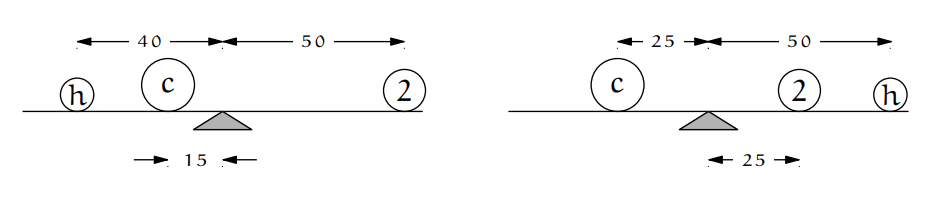
\includegraphics[width=0.8\linewidth]{0-Revisions/2-PivotDeGauss/equilibre.png}
    \end{center}

    \newpage

    \vspace{2em}

    \subsection{Combien de solutions ?}
Ces systèmes admettent-ils zéro, une ou une infinité de solutions ?

\begin{multicols}{3}
\begin{enumerate}[label=\alph*)]
  \item $$\begin{cases}
      -3x + 2y &= 0\\
      -2y &= 0
    \end{cases}$$

  \item $$\begin{cases}
      x + y &= 4\\
      y - z &= 0
    \end{cases}$$

  \item 
  $$\begin{cases}
      x + y &= 4\\
      y - z &= 0\\
      0 &= 0
    \end{cases}$$

  \item 
  $$\begin{cases}
      x + y &= 4\\
      0 &= 4
    \end{cases}$$

  \item 
  $$\begin{cases}
      3x + 6y + z &= -0.5\\
      -z &= 2.5
    \end{cases}$$

  \item 
  $$\begin{cases}
      x - 3y &= 2\\
      0 &= 0
    \end{cases}$$

  \item 
  $$\begin{cases}
      2x + 2y &= 4\\
      y &= 1\\
      0 &= 4
    \end{cases}$$

  \item 
  $$\begin{cases}
      2x + y &= 0
    \end{cases}$$

  \item 
  $$\begin{cases}
      x - y &= -1\\
      0 &= 0\\
      0 &= 4
    \end{cases}$$

  \item 
  $$\begin{cases}
      x + y - 3z &= -1\\
      y - z &= 2\\
      z &= 0\\
      0 &= 0
    \end{cases}$$
\end{enumerate}
\end{multicols}

\vspace{2em}
\subsection{Systèmes d'équations linéaires}
Résoudre les systèmes suivants :

\begin{multicols}{3}
\begin{enumerate}[label={}]
  \item 
  $$\begin{cases}
    2x + 2y = 5 \\
      x - 4y = 0
    \end{cases}$$

  \item 
    $$\begin{cases}
      -x + y = 1 \\
      x + y = 2
    \end{cases}$$

  \item 
  $$\begin{cases}
      x - 3y + z = 1 \\
      x + y + 2z = 14
    \end{cases}$$


  \item 
  $$\begin{cases}
      -x - y = 1 \\
      -3x - 3y = 2
    \end{cases}$$


  \item 
  $$\begin{cases}
      4y + z = 20 \\
      2x - 2y + z = 0 \\
      x + z = 5 \\
      x + y - z = 10
    \end{cases}$$


  \item 
  $$\begin{cases}
      2x + z + w = 5 \\
      y - w = -1 \\
      3x - z - w = 0 \\
      4x + y + 2z + w = 9
    \end{cases}$$

\end{enumerate}
\end{multicols}

\vspace{2em}

\subsection{Approfondissement}
Résoudre 
$$\begin{cases}
    2 \sin \alpha-\cos \beta+3 \tan \gamma &= 3 \\
    4 \sin \alpha+2 \cos \beta-2 \tan \gamma &= 10 \\
    6 \sin \alpha-3 \cos \beta+\tan \gamma &= 9
  \end{cases}$$

  \newpage
  \vspace{2em}

\subsection{Manipulation}

\textit{La méthode de Gauss consiste à combiner les équations d'un système pour en former de nouvelles.}

\medskip
\begin{enumerate}[label=\alph*)]
\item Peut-on obtenir l'équation \(3x - 2y = 5\) par une suite d'opérations de réduction de Gauss à partir des équations de ce système ?
\[
\begin{cases}
x + y = 1 \\
4x - y = 6
\end{cases}
\]

\item Peut-on obtenir l'équation \(5x - 3y = 2\) par une suite d'opérations de réduction de Gauss à partir des équations de ce système ?
\[
\begin{cases}
2x + 2y = 5 \\
3x + y = 4
\end{cases}
\]

\item Peut-on obtenir \(6x - 9y + 5z = -2\) par une suite d'opérations de réduction de Gauss à partir des équations de ce système ?
\[
\begin{cases}
2x + y - z = 4 \\
6x - 3y + z = 5
\end{cases}
\]
\end{enumerate}

\vspace{2em}
\subsection{Interprétation}
Choisir 3 systèmes linéaire dans un exercice précédent et l'écrire des 2 manières différentes : 
\begin{enumerate}
  \item Comme une combinaison linéaires de vecteurs.
  \item Comme une equation matricielle.
\end{enumerate}

Par exemple, le système 
$$\begin{cases}
  x + y = 1 \\
  4x - y = 6
\end{cases}$$
peut s'écrire comme une combinaison linéaire de vecteurs :
$$x\begin{pmatrix}1\\4\end{pmatrix} + y\begin{pmatrix}1\\-1\end{pmatrix} = \begin{pmatrix}1\\6\end{pmatrix}$$
ou comme une equation matricielle :
$$\begin{pmatrix}1&1\\4&-1\end{pmatrix}\begin{pmatrix}x\\y\end{pmatrix} = \begin{pmatrix}1\\6\end{pmatrix}$$

\vspace{2em}
\subsection{Pour ceux qui s'ennuient}
Une boîte contenant des pennies, des nickels et des dimes renferme treize pièces d'une valeur totale de 83 cents.
Combien y a-t-il de pièces de chaque type dans la boîte ?
(Ce sont des pièces américaines : un penny vaut 1 cent, un nickel 5 cents et un dime 10 cents.)
\end{document}
